\chapter{Introduction}
\section{Motivation}
Computer generated music, such as synthsized MIDI, are often considered robotic and unexpressive. But we have already witnessed the fluid and lively sound generated by state-of-the-art text-to-speech systems. This inspired us to develop a system that can read a music score and play it in an expressive, humanly way. Such system can be used for audiolizing score notation editing software, creating interactive media content, and generating royality-free music. 

Established pianists always has his/her own distinctive style. Such sytle distinguised himself/herself from all the other pianists. If the expressive performance system can learn the style of a performer, it might be able to provide musicological insight of performance styles. Furthermore, we can even make a mastero who is no longer with us play music he/she never played in his/her lifetime.


\framebox{TODO:Discuss Mazolla's theroy of expressive performance}

\begin{figure}[tp]
   \begin{center}
      %TODO:Figure: expressive performance concept
      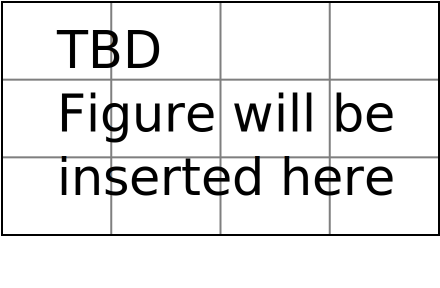
\includegraphics[width=\textwidth]{fig/TBDFigure}

   \end{center}
   \caption{From Composer to Performance}
   \label{fig:concept}
\end{figure}
%Application: musicology study, typesetting tool, play score archive, play computer-generated music, accompaniment



\section{Goal}
The ultimate goal of a expressive performance system is to be able to play any music in a expressive and human-like manner, or even have creative exprssions. But due to the technical and time constrain, we need to define a more pratical goal for our research. We wish to build a computer exprssive performance system based on offline supervised learning. The system will be able to learn any play monophonic melodic phrases. By learning from human recordings, the system will be able to generate expressive performance from previous unseen music notation (also in phrases). The performance style will be controlled by the learning material, if a lot of recordings from different performers are fed in, the system should be able to perform a general human-like expression. If only recordings from a single performer is given, it should learn the particular style of the performer.




\section{Contribution}
The major contribution of this thesis is appling structural support vector machine on expressive performance problem. Also we tried to provide a public corpus for expressive performance. 
%\bibliographystyle{unsrt}
%\bibliography{thesisbib}
\framebox{TODO:Overview of the chapter sctructure of this thesis}
